\documentclass[12pt]{article}

% Packages
\usepackage[utf8]{inputenc}    % For special characters
\usepackage[T1]{fontenc}       % Font encoding
\usepackage{lmodern}           % Enhanced font appearance
\usepackage{float}
\usepackage{amsmath, amssymb, amsthm} % Math packages
\usepackage{graphicx}          % For including graphics
\usepackage{hyperref}          % For hyperlinks
\usepackage{titling}           % For customizing the title page
\usepackage{tocloft}           % For customizing the table of contents
\usepackage{setspace}          % For line spacing
\usepackage{geometry}          % For margins
\usepackage{lipsum}            % For placeholder text
\usepackage[style=authoryear]{biblatex} % More standard footnote citation style

% Add your .bib file
\addbibresource{citation.bib}  % Assumes you have a citation.bib file in the same directory

% Hyperref customizations: enable ToC links but disable red boxes and citation links
\hypersetup{
    colorlinks=true,          % Enable colored text instead of boxes
    linkcolor=blue,           % Color for internal links like ToC
    citecolor=black,          % Color for citation links (black to make them unclickable)
    filecolor=magenta,        % Color for file links
    urlcolor=cyan,            % Color for external links
    pdfborder={0 0 0},        % Removes the border (red box) around links
    hidelinks                 % Hides link colors for citations
}

% Adjustments
\geometry{margin=1in}          % Set margin to 1 inch
\doublespacing                 % Double spacing
\setlength{\droptitle}{-5em}   % Adjusts the space before title (if needed)

% Title information
\title{Researchers Discover Food Dye in Doritos Can Turn Mice Skin Transparent}
\author{Siddarth Kerkar \\ \small{HONR U3310, Contemporary Issues in Healthcare}\\ \small{Professor Lorna Hayward}}
\date{\today}  % Today's date or custom date

% Begin document
\begin{document}

% Vertically center title
\vfill  % Add flexible space above the title

\maketitle

\vfill  % Add flexible space below the title

\newpage

% Abstract
\begin{abstract}
  Recent research has demonstrated that tartrazine, a common yellow food dye, can temporarily render mouse skin transparent when applied topically. 
  This groundbreaking discovery, published in \emph{Science} in September 2024, harnesses principles of optics to reduce light scattering in biological tissues. 
  By matching the refractive indices of different tissue components, the dye allows for non-invasive visualization of internal structures and processes 
  in living animals. This paper examines the scientific principles behind this phenomenon, the experimental methods used, and the potential 
  implications for biomedical research and clinical applications. While the technique has not yet been tested on humans, it shows promise for advancing 
  our understanding of biological systems and improving medical diagnostics and treatments. The paper also discusses the limitations of the current 
  approach and future directions for research in this emerging field of optical tissue clearing.
\end{abstract}
\newpage

% Table of Contents
\tableofcontents
\newpage

% Introduction Section
\section{Introduction}
\label{sec:introduction} 

\subsection{Background}
Tartrazine, commonly known as FD\&C Yellow 5 or E102, is a synthetic lemon yellow azo dye widely used as a food coloring agent. Discovered in 1884 by Swiss chemist Johann Heinrich Ziegler in Basel, tartrazine was patented and produced in Germany by BASF in 1885. Ziegler's work on this new class of dyes was first presented to the scientific community in 1887 in Chemische Berichte, the journal of the German Chemical Society.

\subsection{Use Cases}
Since its discovery, tartrazine has become commonplace in the food industry, finding its way into a variety of products including desserts, confectionery, soft drinks, cereals, and snacks. Its popularity stems from its ability to create vibrant yellow to orange-yellow colors and chemical its stability in various food applications. Moreover, tartrazine is also used in pharmaceuticals, cosmetics, and other consumer products.

While primarily known for its coloring properties, tartrazine has been the subject of ongoing research regarding potential health effects. Some studies have suggested links between tartrazine consumption and allergic reactions or behavioral changes in children, though regulatory bodies like the FDA generally consider it safe for most people when used as directed.

\subsection{New Discovery}
In a surprising development, recent research has unveiled a potentially groundbreaking new application for this common food dye. A study published in Science in September 2024 by researchers at Stanford University and the University of Texas at Dallas demonstrated that tartrazine can be used to make living skin temporarily transparent. By applying a tartrazine solution to mouse skin, researchers created a "window" allowing direct observation of blood vessels, muscles, and internal organs without invasive procedures.

This unexpected application of tartrazine in biomedical imaging showcases how a substance primarily used for its aesthetic qualities can have profound implications in scientific and medical fields. If successfully translated to humans, this technique could revolutionize diagnostic procedures, surgical planning, and our understanding of real-time biological processes.


% Literature Review with In-text Citation Example
\section{Analysis}
\label{sec:analysis}

\subsection{Introduction to the Study}
A groundbreaking study demonstrates a novel approach to rendering living tissues transparent using tartrazine, a common food dye\footnote{Ou et al., "Achieving optical transparency in live animals with absorbing molecules", 2024}. This technique allows for non-invasive visualization of internal structures in live animals, potentially revolutionizing biomedical imaging and research. 

\subsection{Methodology}
The researchers applied a solution of tartrazine (FD\&C Yellow 5) to the skin of live mice, achieving transparency within minutes. This effect was observed in various areas, including the skull, abdomen, and hindlimb\footnote{Ou et al., "Achieving optical transparency in live animals with absorbing molecules", 2024}. The process is reversible, with the skin returning to its original opacity after rinsing with water. 

One of the key advantages of this method is its rapid action. According to the time-lapse images provided in the research (Fig.~\ref{fig:tartrazine}), the mouse scalp transitioned from opacity to transparency within just a few minutes of massaging with tartrazine solution. This quick action is crucial for practical applications in live animal imaging.

%insert Fig
\begin{figure}[H]
    \centering
    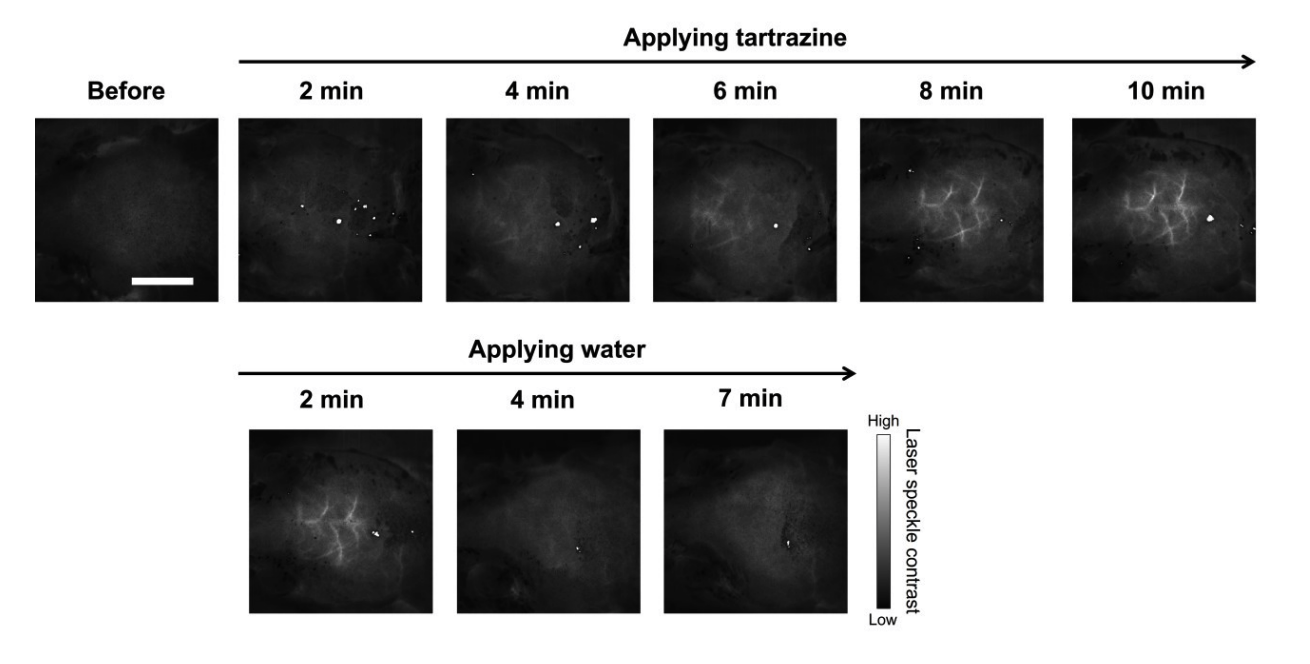
\includegraphics[width=0.9\textwidth]{figures/Applying tartrazine.png}
    \caption{\emph{Time-lapse laser speckle contrast images showing the mouse scalp transitioning 
    from opacity to transparency after applying tartrazine and massaging, and back to opacity after 
    applying water and massaging. Time labels indicate the duration of massaging, not the time since 
    tartrazine or water application. Scale bar: 5 mm.}}
    \label{fig:tartrazine}
\end{figure}


The effectiveness of tartrazine in achieving transparency is attributed to its optical properties. As shown in Fig.~\ref{fig:absorption} of the report, tartrazine exhibits strong absorption in the blue and ultraviolet regions of the spectrum, with peak absorption at 428 nm. This absorption characteristic is key to its ability to modulate the refractive index of tissues.

The researchers explain that tartrazine's effectiveness stems from the Kramers-Kronig relations, which link a material's absorption spectrum to its refractive index\footnote{Ou et al., "Achieving optical transparency in live animals with absorbing molecules", 2024}. By absorbing light in specific wavelengths, tartrazine alters the refractive index of the tissue, reducing light scattering and increasing transparency.


\begin{figure}[H]
  \centering
  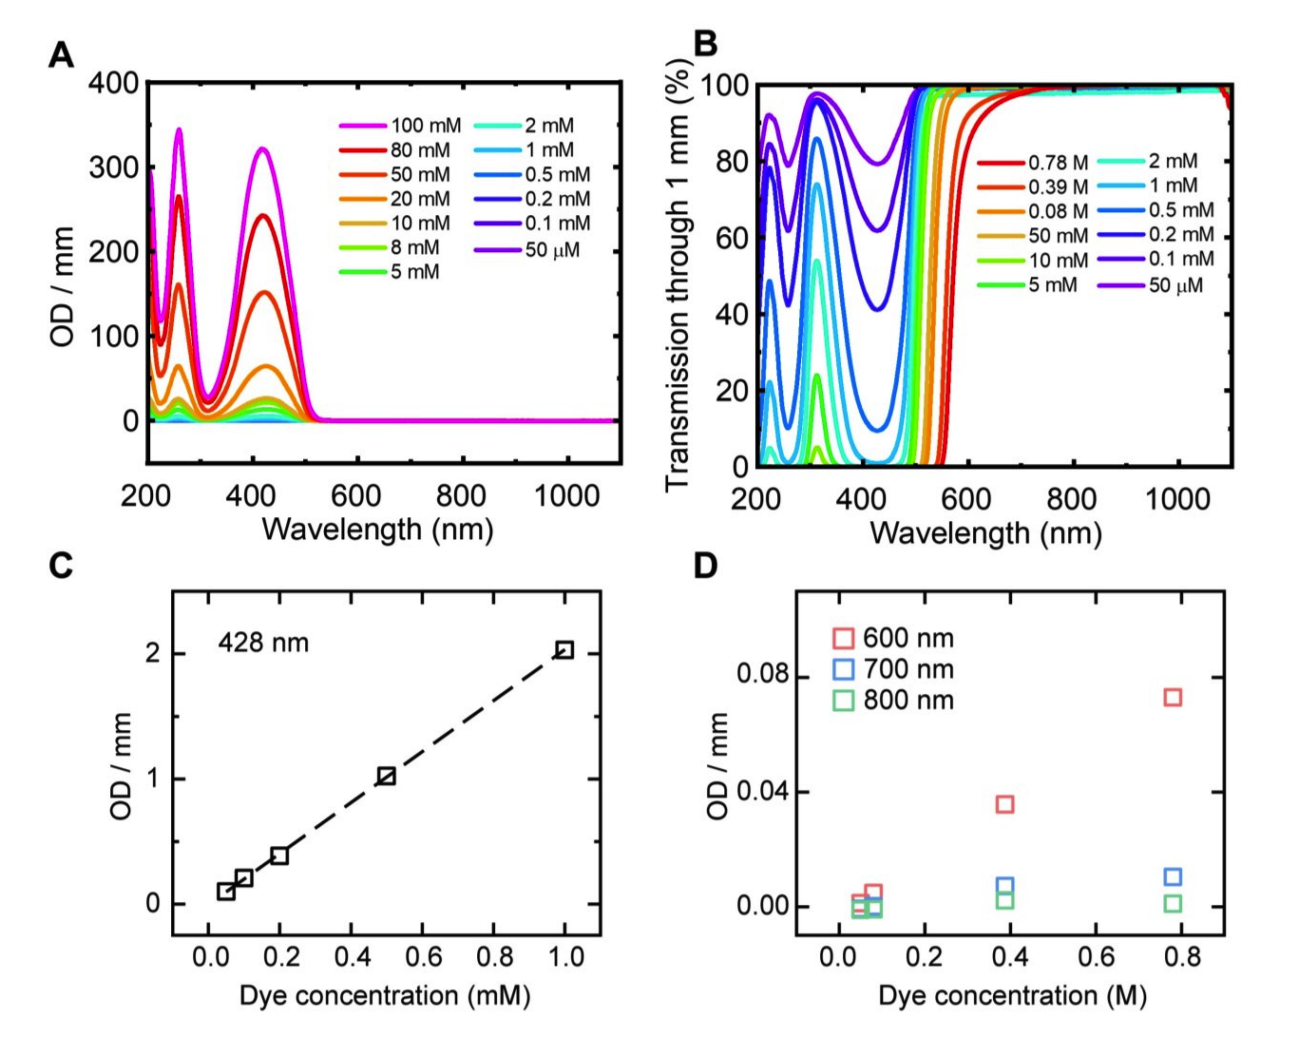
\includegraphics[width=0.9\textwidth]{figures/Tartrazine Light Absorption.png}
  \caption{\emph{Absorption of tartrazine solutions at different concentrations}}
  \label{fig:absorption}
\end{figure}




\subsection{Comparative Analysis}
The study also compared tartrazine to other dyes and conventional \emph{optical clearing agents}. As shown in Fig.~\ref{fig:comparison} of the report, 
tartrazine demonstrated superior performance in terms of its molar refractive ($\Delta$n') index, a measure of determining how much light is transmitted versus scattered.
Tartrazine outperformes glycerol and water for all levels of tickness, $1$ to $5 mm$

\begin{figure}[H]
  \centering
  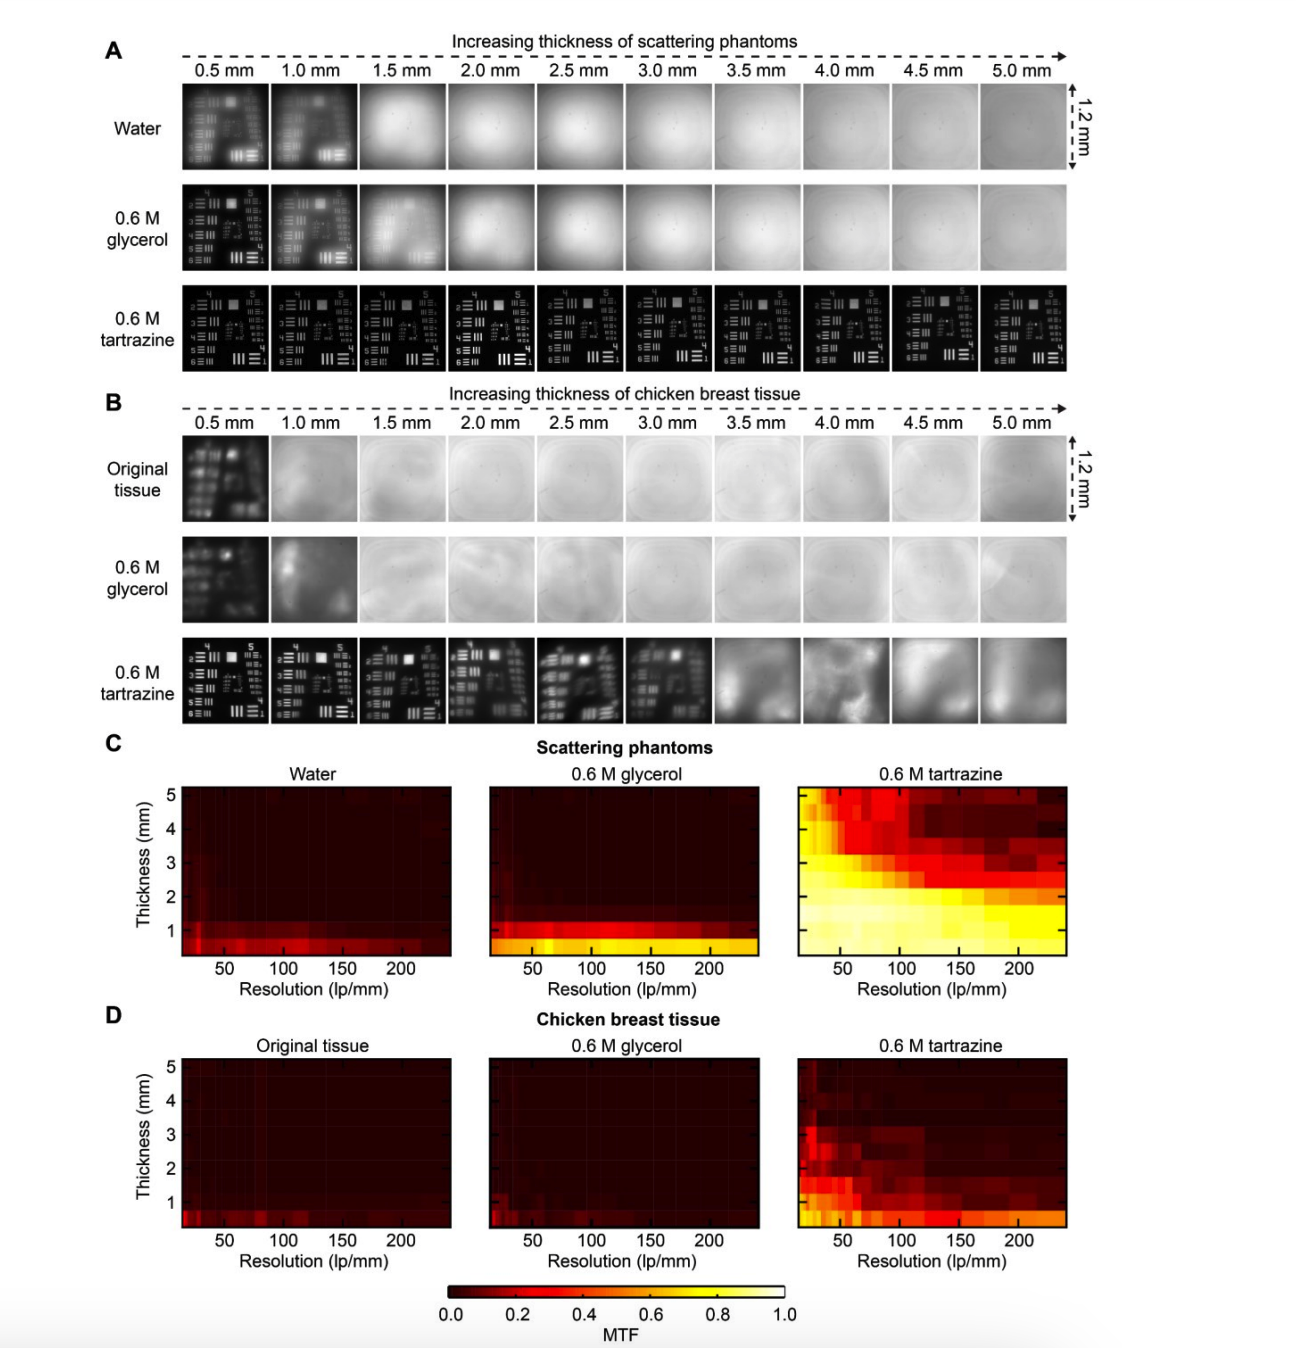
\includegraphics[width=0.9\textwidth]{figures/tartrazine vs gl.png}
  \caption{\emph{Light scattering and absorbtion of tartrazine compared to glycerol and water.}}
  \label{fig:comparison}
\end{figure}



\subsection{Safety}
The researchers conducted extensive tests to validate the safety and long term health effectis of this practice. 
Analysis for potential side effects (Fig.~\ref{fig:health}) showed no signs of inflammation in tartrazine-treated skin samples compared to control samples. 
Additionally, there were little to no discernible differences between the control and tartrazine-treated rats in terms of body weight and blood count (Fig.~\ref{fig:weight} and Fig.~\ref{fig:blood}).


\begin{figure}[H]
  \centering
  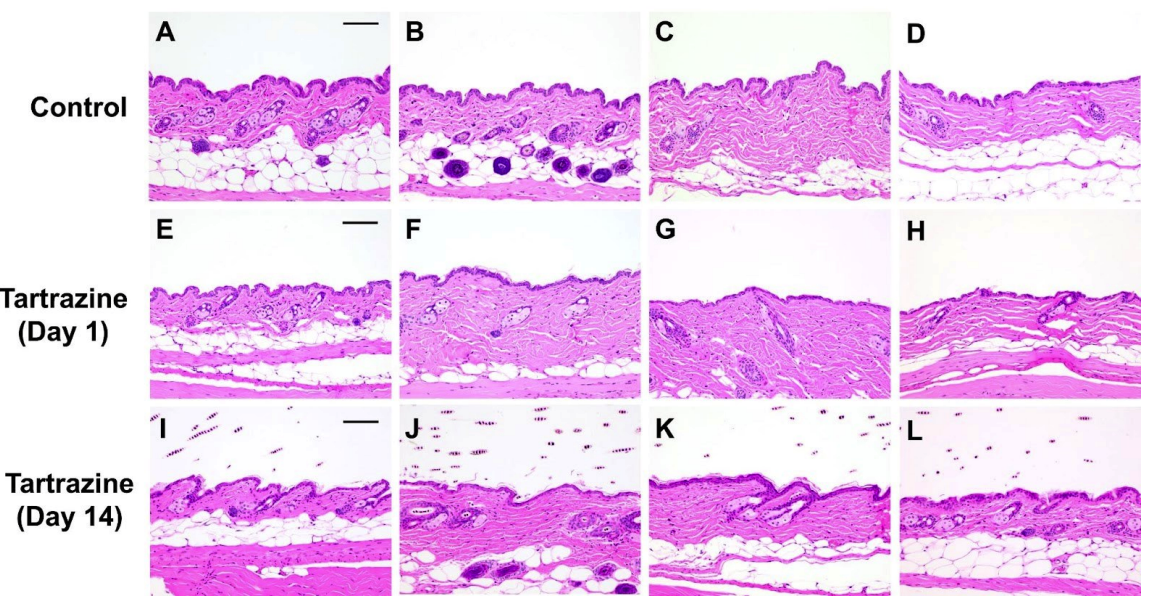
\includegraphics[width=0.9\textwidth]{figures/health.png}
  \caption{\emph{Skin inflammation levels after tartrazine application versus control.}}
  \label{fig:health}
\end{figure}

\begin{figure}[H]
  \centering
  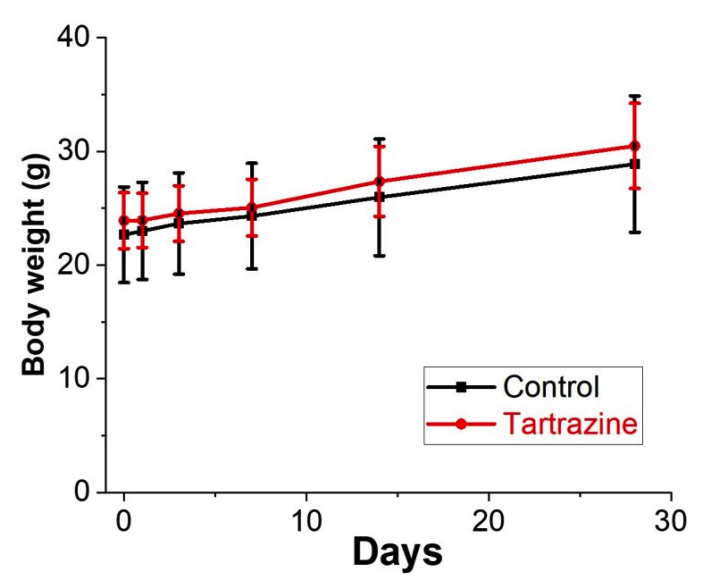
\includegraphics[width=0.6\textwidth]{figures/body weight.png}
  \caption{\emph{Body weight after tartrazine application versus control.}}
  \label{fig:weight}
\end{figure}


\begin{figure}[H]
  \centering
  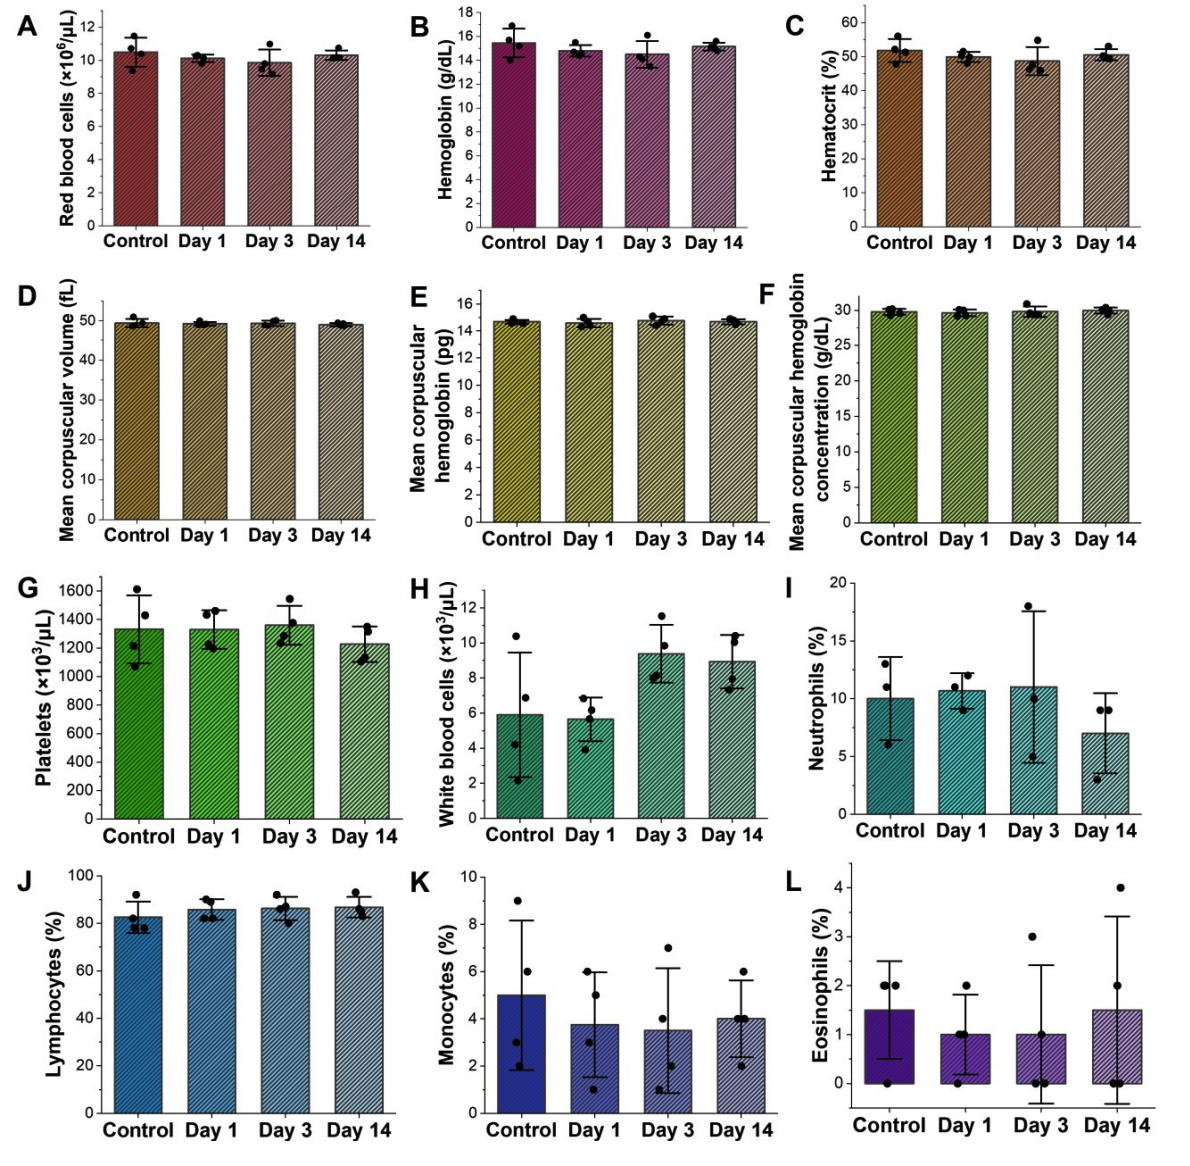
\includegraphics[width=0.9\textwidth]{figures/blood count.png}
  \caption{\emph{Blood count levels after tartrazine application versus control.}}
  \label{fig:blood}
\end{figure}





\subsection{Applications and Implications}
One of the most impressive findings in the study was the ability to see the nerve network in the mouse small intestine through the unbroken abdominal wall\footnote{Ou et al., "Achieving optical transparency in live animals with absorbing molecules", 2024}. 

This non-invasive imaging of deep tissues could greatly impact the study of how the digestive system works and its related diseases.

The potential for human application is still not fully realized, although the researchers note that human skin is about 10 times thicker than mouse skin, which may require adjustments to the overall practice\footnote{Miller, "To turn tissue transparent, dye it yellow", 2024}. The study used concentrations of tartrazine much higher than those typically found in food, emphasizing the need for further safety studies before human trials.


\section{Conclusion}
\label{sec:conclusion}
The study by Ou et al. represents a significant advancement in biological imaging, with potential implications extending beyond basic research to various clinical and adaptive sport applications. By repurposing tartrazine to achieve optical transparency in living tissues, the researchers have opened up new possibilities for non-invasive visualization of internal structures and organ systems in real-time.

This technique could revolutionize preclinical research and enhance clinical diagnostics across multiple fields. In neurology, it might allow direct observation of brain activity through the intact skull. For oncology, it could enable early detection and monitoring of tumors. In developmental biology, it could provide a window into embryonic and fetal development.

\subsection{Adaptive Sports Applications}
Interestingly, this technology could also have applications in adaptive sports. 

Volt hockey, a fast-paced team sport designed for people with limited upper and lower body mobility, such as those with muscular dystrophy, involves players using motorized chairs equipped with paddles. The ability to non-invasively visualize muscle and nerve function could be invaluable for assessing and improving players' performance, as well as for early detection and treatment of sports-related injuries. Moreover, for players who might require surgeries, this transparent skin technique could potentially aid in pre-operative planning and minimally invasive procedures, 
possibly reducing recovery times and allowing players to return to the sport more quickly and remain active. 

\subsection{Limitations}
However, several limitations need addressing. The method's efficacy on human tissues, which are significantly thicker than mouse tissues, remains uncertain. The high concentrations of tartrazine used also necessitate further safety studies before human trials.

\subsection{Future Work}
Future work should focus on optimizing the technique for thicker tissues, exploring its applicability to a wider range of biological systems, and investigating alternative compounds that could achieve 
similar results with lower concentrations. Research into combining this method with other imaging technologies could further enhance its capabilities, potentially benefiting both medical applications and adaptive sports.

While this study marks a significant step forward in biological imaging, considerable research is still needed to fully realize its potential and translate it into practical applications.


% References Section
\newpage
\printbibliography

\end{document}
